\documentclass[10pt]{unlsilabsop}
\title{Destructive wirebond acceptance test of HDI}
\date{September 24, 2014}
\author{Frank Meier Aeschbacher}
\approved{Frank Meier Aeschbacher}
\sopid{209}
\sopversion{v0}
\sopabstract{Describes the procedure to test HDI for suitability to wirebonding. This destructive test is optional and makes HDI not suitable for manufacturing without rworking.}
\begin{document}

\maketitle

%------------------------------------------------------------------
\section{Scope}
This test is mainly for type testing of samples from HDI batches. The test uses ROC wirebond pads to gain large statistics.

HDI can be reworked by removing all traces of wirebonds. Such HDI can be reused without restriction because the normal location of the bond is in the center of the pad whereas this test places it at the two ends of the pad.

%------------------------------------------------------------------
\section{Purpose}
Bondability is a crtical quality criterion for HDI. This test allows to characterize batches of HDI for suitability for wirebonding.

%------------------------------------------------------------------
%\section{Definitions}
%\begin{itemize}
%\item \textbf{bla} Text
%\end{itemize}

%------------------------------------------------------------------
%\section{Responsibilities}

%------------------------------------------------------------------
\section{Equipment}

\begin{itemize}
    \item Wirebonder: Delvotec 56XX
    \item Bond head: Delvotec 5630
    \item Bond wedge: SPT UT45A-W-2030-1.00-C, having a bond flat size of 3\,mils
    \item Pull tester: PH-100
    \item Pull hook: WEP-00001
    \item Chuck
    \item Bond wire: aluminium 25\,$\mu$m diameter, Heraeus ALW-29S on 2" spool
    \item Tweezers for wire handling
    \item Test coupon
    \item In case back side of HDI is too rough to be held by vacuum: Double sided adhesive tape, Scotch 3M 238
    \item Cotton swabs
\end{itemize}

%------------------------------------------------------------------
\subsection{Bonder setting}

Table \ref{tbl:bondpar} lists the bond settings which have to be used by the operator. In order to maintain comparability, using settings other than listed in this table are only allowed upon special request and need explicit mentioning in the test report. Table \ref{tbl:otherpar} lists general machine settings to be used.

\begin{table*}[hH]
\begin{center}
\caption{Bond parameter settings for bonds from HDI to ROC and HDI to sensor HV pad. Bond settings are for both bonds (first and second).}
\label{tbl:bondpar}

\bigskip

\begin{tabular}{lc|c|c}
\toprule
Parameter & Unit & Set A & Set B  \\
    \midrule
US Time      &  ms    &  25 &  50 \\
B-Force      &  cN    &  30 &  30 \\
US Power     & digit  & 140 & 155 \\
TD Steps     & $\mu$m &  12 &  15 \\
    \midrule
Z-Presign    & \%     &  65 &  65 \\
Loop Height  & $\mu$m &   0 &   0 \\
LoopH-Fct    & \%     & 125 & 125 \\
ClampFlag    & --     &   0 &   0 \\
XY LoopH-Fct & \%     &  50 &  50 \\
Z-Delay      & \%     &   0 &   0 \\
   \bottomrule
\end{tabular}
\end{center}
\end{table*}

\begin{table*}[hH]
\begin{center}
\caption{Machine parameter settings. Settings marked with an asterisk (*) may vary according to operator's preference.}
\label{tbl:otherpar}

\bigskip

\begin{tabular}{lcc}
\toprule
Parameter          & Unit   & Value \\
\midrule
Workheight 1       & $\mu$m & 24182 *\\
Workheight 2       & $\mu$m & 36293 * \\
\multicolumn{2}{l}{Use Diagonal Tolerance} & yes \\
Diagonal Tolerance & $\mu$m & 100 \\
TD Ramp            & $\mu$m & 300 \\
Clamp value        & digit  & 650 \\
Feed               & steps  & 16 \\
Limiter            & steps  & 16 \\
Wire Diameter      & $\mu$m & 25 \\
Production Mode    & --     & 1 \\
Adjust Mode        & --     & 1 \\
Bond Mode          & --     & 0 \\
Monitoring Mode    & --     & 0 \\
\midrule
Motor Z max        & $\mu$m & 40800 \\
    \bottomrule
\end{tabular}
\end{center}
\end{table*}

%------------------------------------------------------------------
\subsection{Pull tester settings}
TODO: Deliver this list


%------------------------------------------------------------------
\section{Procedures}

The test consists of two steps: making bonds and pulling them. If more than one sample needs to be tested at once, it is acceptable to first do the wirebonds on all samples and then configure the machine for pull testing.
\begin{enumerate}
    \item Handle bare modules only with proper protection: ESD wristband, gloves, face mask. If HDI are unstuffed, ESD wristband may be omitted.
    \item Configure the bonder for aluminium wedge bonding. Mount the bond head following the manual.
    \begin{enumerate}
	\item Check if bond wire feeds. If in doubt, re-feed wire according to manual.
	\item If bonding for the first time this day: Make a manual test bond on a coupon. Add this to your report.
	\item Check if vacuum is present by reading the gauge. If not, perform the following checks: vacuum pump is on (outside cleanroom), valve is open.
    \end{enumerate}
    \item Depending on how the back side of the HDI has been treated, proceed either way:
    \begin{enumerate}
	\item Place HDI on chuck and turn on vacuum. HDI should be held firmly and no gaps are visible between ROC bond pads and chuck. If not, use alternative approach:
	\item Place double sided adhesive tape over the holes of the chuck and place HDI on it. Press firmly using a cotton swab along the edges. Make sure no other features (wirebonds, surface mounted parts, etc.) present are damaged.
    \end{enumerate}
    \item Identify the HDI and record this information.
    \item Load the bond program named SOP-209-DestructiveHDItesting.db
    \item Run alignment step. Choose one ROC pad and record the number.
    \item Run program. Supervise progress and stop in need, especially when modules are at risk or wirebonds are continuously missing. No stop needed for an occasional miss. Record number of misses per pad group for one ROC.
    \item At the end of the full cycle, check visually if all wirebonds are present. Do not rebond any missing bonds.
    \item Configure the machine for pull testing.
    \item Adjust z-height of the pull hook and set lowest level to a safe height.
    \item Adjust microscope to have the hook and the bond under test in focus.
    \item Make destructive pull tests for $N=25$ wirebonds per ROC pad. The remaining bonds are spares to compensates for missed bonds.
    \item Observe every pull through the microscope and rate the failures according to the scheme given in Fig.~\ref{fig:grading}.
    \item Report the results.
\end{enumerate}

\begin{figure}[h]
    \begin{center}
        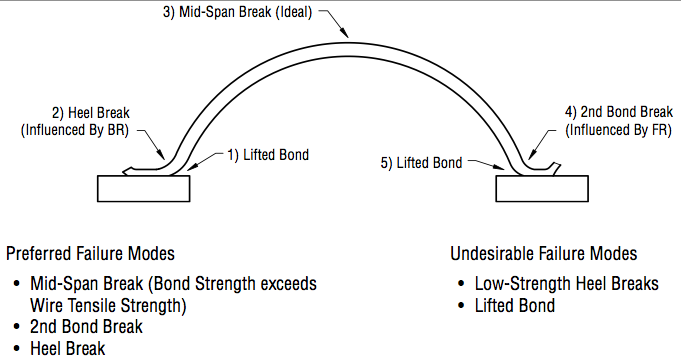
\includegraphics[width=12cm]{img/GradingWedgeBondBreaks.png}
        \caption{Grading of wedge bond breaks. The number signifies the code to be used. Image source: CoorsTek}
        \label{fig:grading}
    \end{center}
\end{figure}

%------------------------------------------------------------------
\section{Documentation}
The following information needs to be recorded in the report for the UNL logbook:
\begin{itemize}
\item Date, time (start--end) and operator name
\item Parameters used
\item Items tested
\item Test results
\end{itemize}


\end{document}

